\subsection{Эшелон Майкельсона}
\begin{figure}[h]
    \centering
    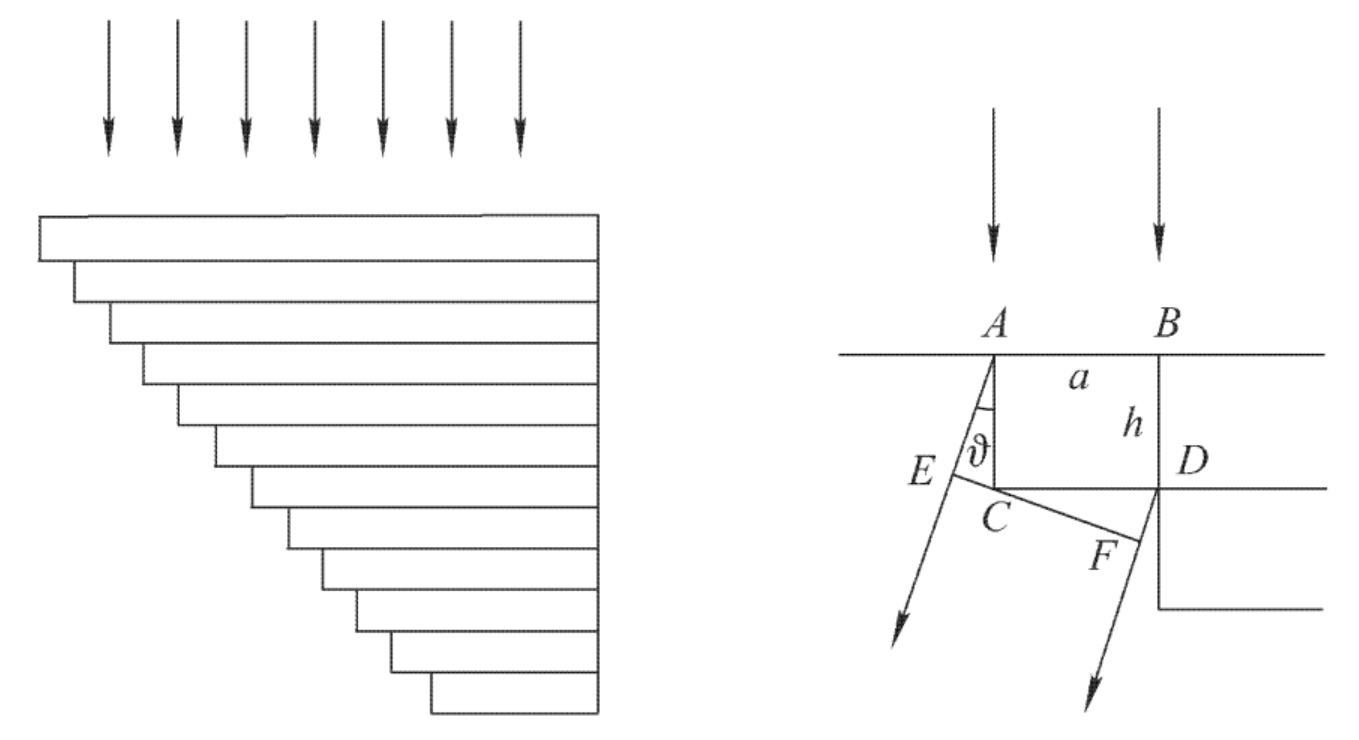
\includegraphics[width=0.45\textwidth]{figures/s47_1.png}
    %\caption{}
    %\label{fig:}
\end{figure}
Для такой картинки разность хода будет:
\begin{equation*}
	\Delta = n h + a \sin \vartheta - h \cos \vartheta = m \lambda.
\end{equation*}
Положения главных максимумов определятся из условия
\begin{equation*}
	nh + a \sin \vartheta - h \cos \vartheta = m \lambda.
\end{equation*}
Найдём дисперсию:
\begin{equation*}
	\frac{d \vartheta}{d \lambda} = \frac{m}{a \cos \vartheta + h \sin \vartheta} \approx = \frac{a}{m} = \frac{h (n-1)}{a \lambda}.
\end{equation*}
Что описывает эшелона как достаточно хороший спектрометр. Его дисперсионная область:
\begin{equation*}
	\Delta \lambda = \frac{\lambda}{m} = \frac{\lambda^2}{h (n-1)}.
\end{equation*}
Она очень мала, что является большим недостатком эшелона.

Разрешающая способность: 
\begin{equation*}
	R = \frac{\lambda}{\delta\lambda} = N m = \frac{N h (n-1)}{\lambda}.
\end{equation*}
Эту формулу можно уточнить, приняв во внимание дисперсию по длине волны от стекла:
\begin{equation*}
	\frac{\lambda}{\delta\lambda} = \frac{N h}{\lambda} \left[(n-1) - \lambda \frac{d n}{d \lambda}\right].
\end{equation*}
И аналогичные аналогичными рассуждениями:
\begin{equation*}
	\Delta\lambda = \frac{\lambda}{m - h (d n / d\lambda)},
	\hspace{0.5 cm}
	\frac{d \vartheta}{d \lambda} = \frac{m - h (d n/d \lambda)}{a \cos \vartheta + h \sin \vartheta}.
\end{equation*}	